\documentclass{llncs}
%Packages 
%\usepackage{amsmath}
\usepackage{fancyhdr}
\usepackage{float}
%\usepackage{caption}
%\usepackage{graphicx}
%\usepackage{placeins}
\usepackage{listings}
\usepackage{pdfpages}
\usepackage{url}
\usepackage[hidelinks]{hyperref}
\usepackage[titletoc]{appendix}

%Settings 
\restylefloat{table,figure}
\graphicspath{{images/}}
\pagestyle{headings}
\pagenumbering{arabic}
\bibliographystyle{abbrv}
% Listing settings start
\renewcommand{\lstlistingname}{Code Sample}
\lstset {
    basicstyle = \footnotestyle\ttfamily,
    captionpos = b,
    breaklines = true
}
% Listing settings end

%Fix TOC
% make a proper TOC despite llncs
\setcounter{tocdepth}{2}
\makeatletter
\renewcommand*\l@author[2]{}
\renewcommand*\l@title[2]{}
\makeatletter
%End fix TOC

%Meta
\title{CUDA GPGPU programming using F\# Alea.cuBase and Actulus CalcSpech for parallelized pension reserve estimation}
\author{Nicolai Skovvart \email{nbsk@itu.dk}\\Superviser: Peter Sestoft}
\date{\today}
\institute{IT University of Copenhagen}

%Document 
\begin{document}
	
	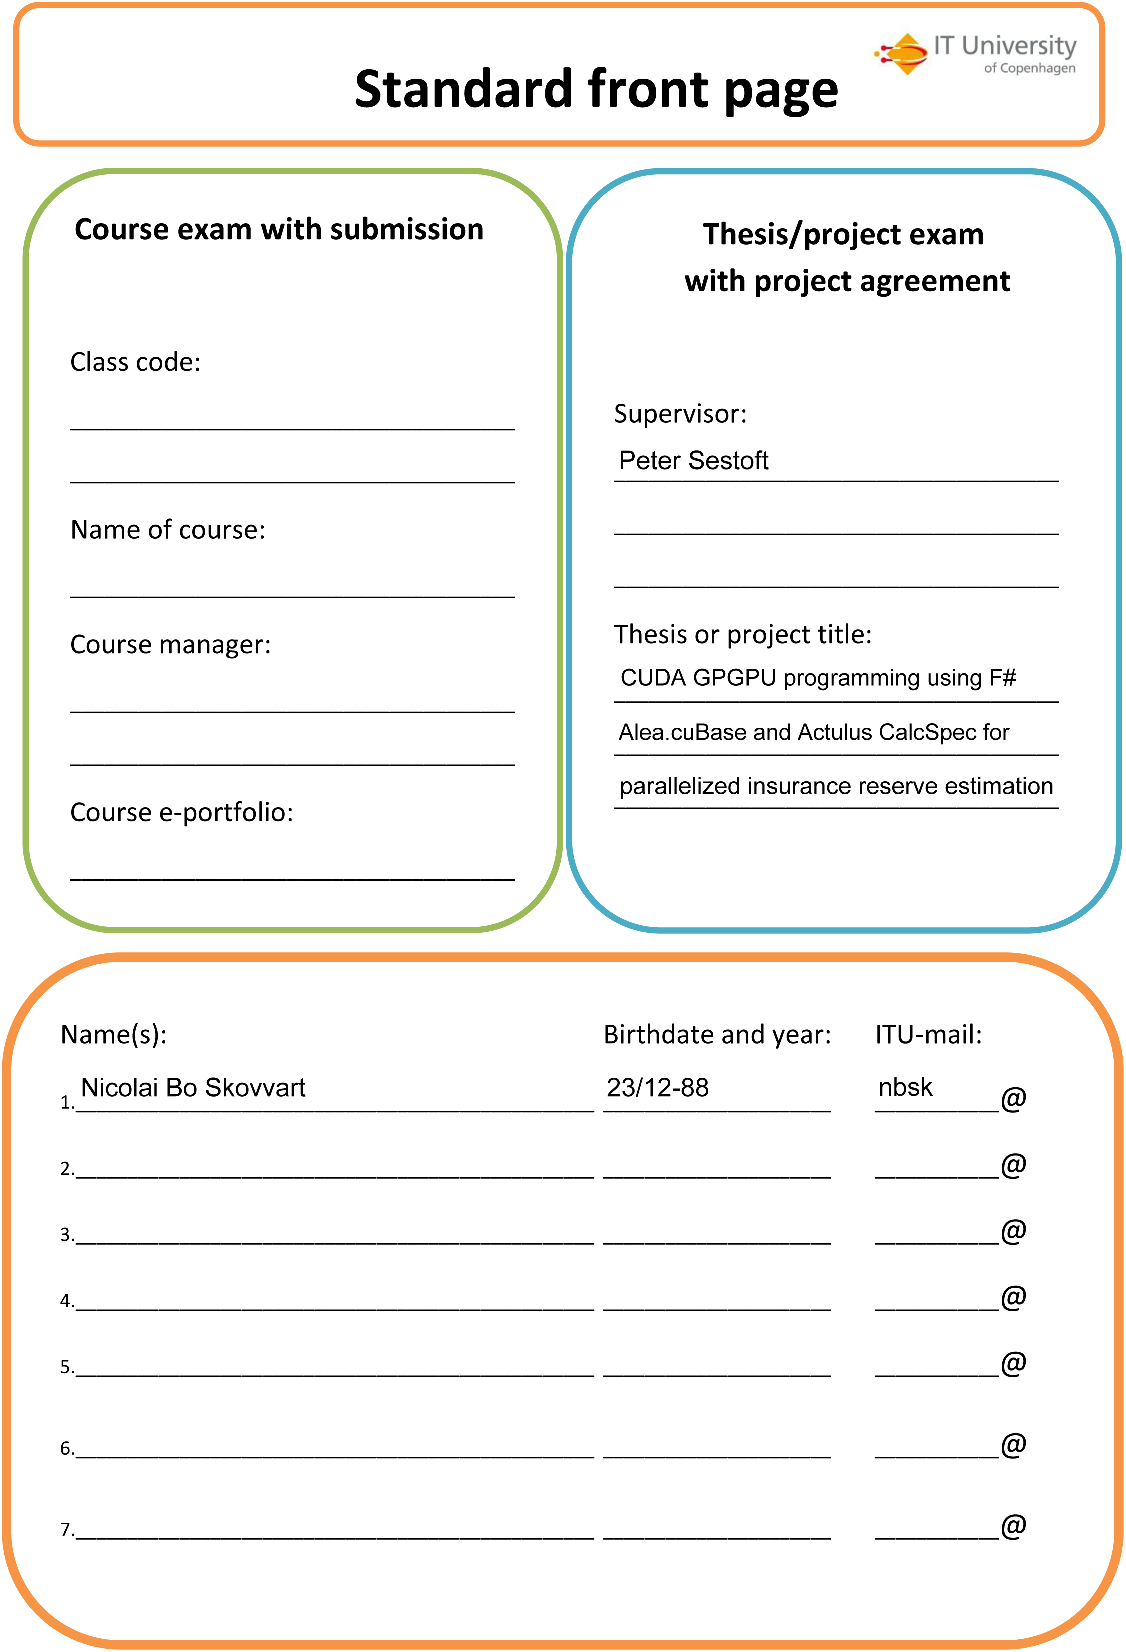
\includepdf[pages={1}]{sections/FrontPage.pdf}
	\setcounter{page}{1}
	
	\maketitle

	% !TeX root = ../thesis.tex
\begin{abstract}
Parallelization can provide great performance boosts for large-scale independent numerical computations, for example in the field of insurance reserve estimation.
NVIDIA's CUDA platform allows for utilization of the parallelization power of the Graphic Processing Unit (GPU), but development is typically done using the CUDA C language which is based on the somewhat archaic C and C++ languages.
Industry would also benefit from being able to utilize the power of the GPU on modern platforms such as Microsoft's .NET.

This thesis investigates the benefits of transforming a single-threaded insurance reserve estimator to utilize parallelization on the GPU on the CUDA platform.
A base-line implementation is done in CUDA C and is then ported to the newer F\# language with the aid of the language integrated compiler Alea.cuBase and the performance implications are explored.
The F\# solution is further enhanced with the capability of parsing insurance plans written in Actulus CalcSpec that are automatically transformed into F\# Alea.cuBase GPU code. The performance implications of this is also explored.

The thesis concludes that software such as insurance reserve estimators can greatly benefit from parallelization on the GPU and that the benefits of developing on a modern platform such as F\# far outweigh the costs.
The parallelized version is up to 2400 times faster than the single-threaded version allowing for many more variations of the insurance plans.
It is also discovered that GPU code automatically transformed from calculation specifications barely have any negative consequences on performance or expressiveness.

\keywords{GPU Parallelization, Language Transformation, Insurance Reserve Estimation, F\# Alea.cuBase, Actulus CalcSpec, CUDA C}
\end{abstract}

	\tableofcontents
	\listoffigures

	\clearpage	

	% !TeX root = ../thesis.tex
\section{Introduction}
As Central Processing Unit (CPU) clock-rate growth have mostly stagnated in the recent century due partially to power inefficiency (\textbf{(QUOTE - \url{http://spectrum.ieee.org/computing/hardware/why-cpu-frequency-stalled} or \url{http://en.wikipedia.org/wiki/Frequency_scaling}?}), parallelization is seen as one of primary techniques for speeding up applications.

While parallelization can be utilized by multi-core CPUs, General Purpose Graphics Processing Units (GPGPU's) in particular are used when computations on large amounts of data is needed, despite originating from the Graphics Processing Unit (GPU) designed for performing calculations in relation to computer graphics.

Parallelization is especially useful for large amounts of independent calculations that can be found in financial fields such as banking or pension.

GPGPU programming is often done on the Compute Unified Device Architecture (CUDA) platform by NVIDIA \cite{NVIDIA}. 
The CUDA platform supports multiple languages, for example as Python and Fortran, it is primarily used by NVIDIA's CUDA C (\textbf{QUOTE}) which is based on the somewhat archaic C/C++ languages.

In this thesis a single-threaded C\# pension reserve estimator will be be translated to the CUDA platform and parallelized and performance gains will be explored and analyzed.
First a base-line implementation will be done in CUDA C and later a solution will be implemented on the more modern .NET platform in the F\# language using the language-integrated compiler Alea.cuBase.
This is to allow for more rapid development utilizing GPGPU parallelization as well as allowing it to be incorporated in a .NET work-flow.

%designed to rapidly manipulate and alter memory

\subsection{Reading guide}
Subjects will be described in various levels of detail depending on their relevance to the main topics of the thesis.
This means that certain languages and paradigms will be described in less detail than strictly required background information and solution descriptions.

The thesis is structured in the following chapters.

The first chapter will introduce the thesis, including the motivation, the scope and approach/method used.

The second chapter will cover a lot of the background knowledge including the math used, parallelization in general and how the GPU facilitates it, the CUDA platform and the CUDA C language, the F\# language and the language integrated compiler Alea.cuBase.

The third chapter will cover descriptions of the various implemented solutions, starting with the initial single-threaded C\# solution, followed by the ''native'' CUDA C implementation and finally the solution in F\#/Alea.cuBase.

The fourth chapter will describe how pension plans written in Actulus CalcSpec are parsed and transformed to F\#/Alea.cuBase kernels and the performance ramifications of this.

The fifth chapter will discuss how various alterations to the project affected performance and discuss their viability. These alterations include adding customer and pension plan variables, various memory types and the order of execution and various optimization strategies are attempted.

The sixth chapter will discuss similarities and differences to related work.
Finally, the seventh chapter will conclude the thesis.
	% !TeX root = ../thesis.tex
\section{Background}
The background section will cover eight topics.
First insurance policies in general will be explained.
Following this, the mathematics employed in this project will be covered. 
This consists of Thiele's differential equation and the fourth-order Runge-Kutta method for solving differential equations.

After the mathematics is covered, the technologies utilized will be presented.
First general information on parallelization and the potential benefits of using the GPU compared to the CPU will be explained.
The CUDA platform and CUDA C will then be presented.
This is followed by an introduction to F\#'s meta-programming model Code Quotations which is used by the language-integrated compiler Alea.cuBase to generate GPU code.
The syntax of the Actulus Calculation Specification (CalcSpec) language will then briefly be explained.
Finally, the hardware the project has been tested on will be presented.

\subsection{Life Insurance Policies and Markov-models}
A life insurance policy is a contract stating the obligations an insuring party has to an insured party in and transitioning between various finite states over many years.
Such states can include being alive and well (active), disabled, dead and more.
Transitions between states will have a certain probability, for example mortality rates for transitions between the active and dead state.
A state model such as this is also known as a continuous-time Markov-model which is used for both its expressiveness and its analyzability.

Figure \ref{fig:markovexample} shows an example of such a model with 3 states and 3 transitions between states. More or less of both are possible.
The labels between the states each have a $\mu$-function that states the probability of the transition occurring at time $t$. 
This is also known as the transition intensity.
Not all transition intensities will change over time while others such as mortality rate will.
For each change in time $t$ to $t+1$ there may be associated costs whether there is a state transition or not.

\begin{figure}[h] 
\setlength{\unitlength}{0.14in} % selecting unit length 
\centering % used for centering Figure 
\begin{picture}(20,8) % picture environment with the size (dimensions) 
 % 32 length units wide, and 15 units high. 
\put(3,6){\framebox(6,3){0 (Active)}} 
\put(13,6){\framebox(6,3){1 (Disabled)}}
\put(8,0){\framebox(6,3){2 (Dead)}} 

\put(6.2,6){\vector(1,-1){2.9}}
\put(9,7.5){\vector(1,0){3.9}} 
\put(16.2,6){\vector(-1,-1){2.9}}

\put(9.5,8.5) {$\mu_{01}(t)$}
\put(15,4) {$\mu_{12}(t)$} 
\put(4.5,4) {$\mu_{02}(t)$} 
\end{picture} 
\caption{Disability Term Insurance Markov-model example} % title of the Figure 
\label{fig:markovexample} % label to refer figure in text 
\end{figure} 

\subsection{Thiele's differential equation and the Runge-Kutta Method}
The goal of the computations performed in this thesis is to estimate the amount of money (reserve) required to be able to fulfil the obligations of a given life insurance plan.
Thiele's differential equation called ``the foundation of modern life insurance mathematics''\cite{bergermathematik} is a tool for determining conditional expected values in Markov models and it can be used to express a variety of life insurance policies.
The equation is expressed below in equation \ref{eq:thiele}. It assumes continuity for $V_s$, $b_s$, $\mu$ for every $t$ and consists of the following parts:

\begin{itemize}
\item $S$ is the total amount of states
\item $V_s(t)$ is the reserve at time $t$ in state $s$
\item $r_s(t($ is interest-rate at time $t$ in state $s$
\item $b_s(t)$ is the benefit paid by the insurer at time $t$ in state $s$
\item $T_s(t)$ is the possible transitions in state $s$
\item $\mu_{s,ts}(t)$ is the transition intensity from state $s$ to state $ts$
\item $b_{s,ts}(t)$ is the transition cost from state $s$ to state $ts$
\end{itemize}

\begin{equation}\label{eq:thiele}
\frac{d}{dt}V(t) = \forall_{s\in S} r_s(t) V_s(t) - b_s(t) - \sum_{ts \in T_{s}} \mu_{s,ts}(t) (V_{ts}(t) - V_s(t) + b_{s,ts})
\end{equation}

To shortly summarize it, the derivative reserve is for all states the current reserve times the interest-rate minus the benefit paid by the ensurer in the state minus the weighted transitioning costs to all possible states. 
The weighted transitioning cost to a state is the intensity of the transition (probability of the transition occurring) times the difference in reserves plus the cost of transitioning.

With a differential equation such as this, we need a way to approximate a result numerically. 
The Runge-Kutta method\cite{press2007numerical} is a method for integrating ordinary differential equations (ODEs) by using a trial step at the midpoint of an interval to cancel out lower-order error terms.
It works within boundaries set by a starting and end point. If the starting point is greater than the end point, the algorithm works backwards with negative step-sizes.
The basic implementation uses a fixed amount of steps to reduce the inaccuracy of the method. 
By increasing the amount of steps, the inaccuracy of the method is reduced at the cost of increased computational costs.
The most common step size seen in this project is 100 steps by advice of Peter Sestoft and by calculation specification definitions.
The fourth-order version of the Runge-Kutta method can be seen below in equation \ref{eq:rk4} approximating $y$ in the step from $t$ to $t+h$. It consists of the following parts:

\begin{itemize}
\item $h$ is the size of the step. With 100 steps, the step-size would be 0.01, or -0.01 if the start point $>$ end point.
\item $f(t, e)$  is the right hand side of the given differential equation evaluated at time $t$ in environment $e$
\item $t$ is the initial time of the step
\item $y_t$ approximated result at time t
\item $O(x)$ represents the inaccuracy of the method
\end{itemize}

\begin{equation}\begin{aligned}\label{eq:rk4}
&k_1 = h f(t, y_t)\\
&k_2 = h f(t + \frac{h}{2}, y_t + \frac{k_1}{2})\\
&k_3 = h f(t + \frac{h}{2}, y_t + \frac{k_2}{2})\\
&k_4 = h f(t + h, y_t + k_3)\\
&y_{n+1} = y_t + \frac{k_1}{6} + \frac{k_2}{3} + \frac{k_3}{3} + \frac{k_4}{6} + O(h^5)
\end{aligned}\end{equation}

%Insert graphics showing step

\subsection{Parallelization and the GPU}
Parallelization is the act of taking one large task and splitting it into smaller tasks that run concurrently (''in parallel'').
This could for example be cooking 10 different pies, where rather than using 1 baker in 1 kitchen you now use 10 bakers in 10 kitchens taking approximately a tenth of the time.
Algorithmically this could be an algorithm that initially does some computation that loops $n$ times where each iteration is independent and takes $w$ time to complete, but is altered to instead utilize $n$ tasks that each execute one iterations worth of work.
Instead of taking $w \cdot n$ time to complete, it can now be done in just $w$ time plus whatever overhead is associated with creating the tasks and dividing the work.
This is reliant on each iteration being independent, as if the iterations are dependent on each other then it can not be executed before the previous iteration completes.
To continue the pie example, if one baker is assigned to make all the pie-crusts, no pie will be baked before this tasks is done.
Loops isn't the only way to utilize parallelization and all independent tasks can to some extend be parallelized. 
Utilizing various synchronization techniques, partially dependent calculations can also harness the power of parallelization, though at the risk of increased complexity and errors such as deadlocks.
As only independent computation parallelization is utilized, other forms will not be discussed further.

In computing, parallelization utilizing constructs such as processes and threads can be performed on multi-core CPUs, but can especially be utilized by GPUs that were designed for compute-intensive and highly parallel computations, precisely what graphics rendering is about.
This is because unlike the CPU which is specialized for data-caching and flow control, the GPU has more transistors dedicated to data processing as illustrated in green by figure \ref{cpugpu}. 
The figure contains Arithmetic Logic Units (ALU's, in green) responsible for logical operations and integer arithmetic, Control Units (in yellow) responsible for communication and coordination between input/output devices and various memory units (in orange) such as a memory cache and dynamic random-access memory (DRAM).

\begin{figure}[h!]
\includegraphics{cpugpu.jpg}
\caption{Structural comparison of the CPU and GPU. From the CUDA C Programming Guide, page 3 \cite{nvidia2014programming}\label{cpugpu}}
\end{figure}

\subsection{The CUDA platform and CUDA C}
CUDA is NVIDIAs parallel computing platform and programming model for the GPU.
It is available on multiple platforms but does require an NVIDIA graphics card. 
A particular NVIDIA graphics card will have a certain Compute Capability (CC) that determines availability of certain attributes and features.

The CUDA platform consists of the CUDA C and C++ language (referred to as CUDA C from this point), based on the C and C++ languages but with some alterations.
It also has parallel computing extensions for other languages such as Fortran and Python.
The CUDA Toolkit is also a part of the platform, consisting of a compiler, math libraries and tools for debugging and optimizing performance as well as guides, user manuals, API references and other documentation.

\subsubsection{CUDA Architecture}
The CUDA model is build around a hierarichal architecture of the GPU. 
At the top of the architecture is the streaming multi-processor (SM) of which a GPU can have many. 
Each SM consists of multiple CUDA cores that are used to concurrently execute a group of 32 threads known as a warp. 
As the SM executes the instructions in terms of warps, the total amount of threads in a block should be a multiple of the warp-size for maximum efficiency.
Each SM executes one group of threads that have access to a shared memory-space.
This group of threads, which ideally should be a multiple of warps, is called a block. 
An example overview of the architecture can bse seen in figure \ref{cuda_architecture}.
As each SM executes blocks sequentially, more SMs available to the GPU will increase the possible parallelization and speed up the execution of the total amount of blocks. 
This also means that the amount of blocks should be a multiple of the amount of multiprocessors for maximum efficiency.

\begin{figure}[h!]\centering
\includegraphics[scale=0.75]{cuda_architecture.jpg}
\caption{The CUDA SM/block architecture. From the CUDA C Programming Guide, page 7 \cite{nvidia2014programming}\label{cuda_architecture}}
\end{figure}

\subsubsection{Thread Hierarchy}
Blocks can be organized in a grid of multiple dimensions (up to 3 on the latest version of NVIDIA cards). 
The same applies to the threads within a block.
An example of can be seen in figure \ref{thread_distribution}.

\begin{figure}[h!]\centering
\includegraphics[scale=0.75]{thread_distribution.jpg}
\caption{The CUDA thread hierarchy. From the CUDA C Programming Guide, page 11 \cite{nvidia2014programming}\label{thread_distribution}}
\end{figure}

As this project only utilizes 1-dimensional grids and blocks, the resulting thread hierarchy is a two-dimensional matrix. 
An example with the unique thread-id's can be seen in figure \ref{thread_hierarchy}.

\begin{figure}[h!]\centering
\includegraphics[scale=0.75]{thread_hierarchy.jpg}
\caption{1-dimensional CUDA thread hierarchy.\label{thread_hierarchy}}
\end{figure}


\subsubsection{Memory model}
A thread has access to various types of memory.
There is local memory only available to the thread itself.
This is facilitated by a relatively small amount of fast registers as long as they are available and falling back on relatively slow local memory afterwards (stored in global memory but only accessed by the thread).

Beyond that, it has access to low-latency shared on-chip memory physically residing on the GPU that is available to all threads in the same block. 
Because of these properties, shared memory can be used for communication between threads or as a software managed cache.

The thread also has access to global off-chip memory accessible to all threads in all blocks.
This has a higher latency, but caching can alleviate some of this.

There is also 64KB of immutable cached constant memory which can be an alternative to unchanging global memory.
It is especially fast when all threads in the warp need to read the same memory location.
Constant memory will often be faster than global memory due to a higher likelihood of being cached on-chip, but the fact it is immutable and of a fixed size limits its applicability.
Another immutable memory type is texture memory which can be used for various purposes, but is ideally used for algorithms with memory access patterns where threads are likely to read from an address that is 2-dimension-spatially local (such as computer graphic shaders).

Data loaded from local or global memory is cached in the on-chip L1 cache for each SM and a shared L2 cache for all SMs.
The L1 cache will typically contain up to 16KB of data, but this limit can be increased up to 48KB by by sacrificing shared memory.
The L2 cache will on newer graphics cards contain up to 768KB of data.

A summary of the properties of the various memory types can be seen in table \ref{table:memorytypes}.

\begin{table}[h!]
\centering
\begin{tabular}{ | c | c | c | c | c | }
  \hline
           & Read-only & On-chip   & Cached & Scope  \\ \hline
  Register & No        & Yes       & No     & Thread \\ \hline
  Local    & No        & No        & Yes    & Thread \\ \hline
  Shared   & No        & Yes       & No     & Block  \\ \hline
  Global   & No        & No        & Yes    & Kernel \\ \hline
  Texture  & Yes       & No        & Yes    & Kernel \\ \hline
  Constant & Yes       & No        & Yes    & Kernel \\ \hline
  L1 Cache & No        & Yes       & N/A    & N/A    \\ \hline
  L2 Cache & No        & No        & N/A    & N/A    \\ \hline

\end{tabular}
\caption{Properties of CUDA memory types\label{table:memorytypes}}
\end{table}

\subsubsection{CUDA C}
CUDA C is based on C with added declaration specifiers for methods and variables. 
The most essential declaration specifier is the \textbf{\_\_global\_\_} specifier which declares a method to be a \textbf{kernel}. 
Kernels are void-methods that are callable from the CPU but executed on the GPU. 
Code sample \ref{cuda_add} shows a simple kernel performing vector addition of the vectors $a$ and $b$ of size $N$.

\begin{lstlisting}[language=C++, caption=CUDA C addition kernel, label=cuda_add]
__global__ void Add(float* a, float* b, float* result){
	//unique id within the kernel
	int i = threadIdx.x + blockIdx.x * blockDim.x;
	// (blockIdx always 0 in this example)
	result[i] = a[i] + b[i];
}

int main(){
	...//Initiate memory on host and device
	Add<<<1, N>>>(a, b, result); //invoke kernel on 1 block of N threads
	...//Copy back and use result, free memory as appropriate
}
\end{lstlisting}

One thing to note is the kernel launch-parameters of Add-method in $main$ which specify the amount of blocks and the amount of threads per block on which the kernel should be executed. 

CUDA C also has other declaration specifiers. 
\textbf{\_\_device\_\_} specifies that a method will only be compiled for the GPU (which can be referenced by kernels), \textbf{\_\_host\_\_} specifies that a method will be available for the CPU.
These two specifiers can also be used together for compilation to both platforms.
Variables have the \textbf{\_\_device\_\_} qualifier, as well as \textbf{\_\_constant\_\_} to indicate it should be stored in constant memory or \textbf{\_\_shared\_\_} for shared memory.

As it is based on C, dynamic memory must be allocated using $malloc$ and subsequently de-allocated by $free$.
This operation also has to be done for the device memory using the equivalent $cudaMalloc$ and $cudaFree$.
The tediousness of this is one of the many benefits of using a modern language, but at the cost of control that could potentially decrease performance.

\subsection{F\# and Code Quotations}
F\#\cite{fsharp} is an open source, cross-platform functional programming language originating from Microsoft that runs on the .NET platform.
Code quotations is a language feature of F\# that allows one to dynamically generate abstract syntax trees from F\# expressions. 
It is used in particular to transform F\# to other languages such as SQL automatically. 
It can also be used to generate F\# code that can be evaluated. 
Code quotations support both typed and untyped expressions using $<@ ... @>$ and $<@@ ... @@>$ respectively. 

For example, the expression $<@ let plusfive number = number + 5 in plusfive @>$ is automatically translated into the abstract syntax tree in figure \ref{quotationast}. 
As quotations only support expressions, a let declaration can not exist on its own, hence returning the function at the end (in the $in$ part of the quotation).

\begin{lstlisting}[caption=Abstract syntax tree for the example quotation expression, label=quotationast]
Let (plusfive, 
	Lambda (number, 
		Call (None, op_Addition, [number, Value (5)])
	), 
	plusfive)
\end{lstlisting}

Code quotations also allow for the mixing of quotation expressions using the splicing operators $\%$ for typed and $\%\%$ for untyped expressions as can be seen in code sample \ref{quotationsmixin}.

\begin{lstlisting}[caption=Quotation mixing, label=quotationsmixin]
let plusfive = <@ let plusfive number = number + 5 in plusfive @>
//Has type Expr<int->int>
let plus10 = <@ let plusten number = number |> %plusfive |> %plusfive in plusten @>
//Also has type Expr<int->int>
let untypedplus10 = <@@ %plus10 @@>
//Has type Expr
\end{lstlisting}


\subsection{F\# and Alea.cuBase}
Alea.cuBase by QuantAlea\cite{quantalea} is a commercial language-integrated compiler for F\# that allows for CUDA development on the .NET platform.
By relying on run-time code-generation it allows for extremely extensible kernels to an extend not easily possible in CUDA C.

It utilizes F\#'s meta-programming support Code Quotations for automatic run-time generation of abstract syntax-trees that are then compiled into CUDA's Instruction Set Architecture (ISA) Parallel Thread Execution (PTX) code using Alea.cuBase's compilation API.
Code sample \ref{cubase_add} shows what a simple vector squaring-kernel could look like in F\# using Alea.cuBase.

\begin{lstlisting}[caption=Alea.cuBase square kernel, label=cubase_add]
let Square = cuda { //use the Alea.cuBase cuda workflow
  let! kernel = <@ fun (a:deviceptr<int>) (result:deviceptr<int>) ->
      let i = blockIdx.x * blockDim.x + threadIdx.x
      result.[i] <- a.[i] * a.[i] @> |> Compiler.DefineKernel
  return Entry(fun program ->
    let worker = program.Worker
    let kernel = program.Apply kernel
    //return host-execution method
    fun (a:int[]) ->
      use a = worker.Malloc(a)
      use result = worker.Malloc(Array.zeroCreate a.Length)
      kernel.Launch (LaunchParam(1, a.Length)) a.Ptr result.Ptr
      result.Gather()) //return result
}
[<EntryPoint>]
let main argv = 
  let a = [| for i in 1 .. 10 -> i |]
  use program = Square |> Compiler.load Worker.Default
  program.Run a |> Array.iter (fun e -> printfn "%d" e)
  0 //return 0 to indicate success
\end{lstlisting}

The $cuda$ workflow/computation expression (or ``monad'' for the so inclined) contains the kernel defined in a code quotations and compiled to an actual kernel, and it returns a host-side execution method that will handle allocation and de-allocation of device-side memory. 
As we are using F\#, the deallocation is handled automatically by using the $use$-keyword that automatically frees up resources once the variables referencing them are out of scope. 
The kernel is then loaded to a worker (a CUDA context and background-thread) in the main method compiling the PTX code to NVIDIA internal ISA code. %explain better
The kernel is then run using the parameters defined in the run-time method of the $cuda$ workflow (in this case, just an integer array) and the result is returned to the CPU where it can be processed (only printed to the console in this example).

\subsection{Actulus Calculation Specification language}
The Actulus Calculation Specification language (CalcSpec) is a domain-specific language for defining the differential equations that make up an insurance plan.
The main purpose of the language is to define various coefficient used in the Markov-model defining the life insurance policy.
The overall structure of the language can be seen in code sample \ref{calcspecstructure}.

\begin{lstlisting}[caption=CalcSpec structure, label=calcspecstructure]
calculation = {
    name = <Name of calculation>,
    algorithm = { <Algorithm> },
    equations = { <Equations> },
    range = { <Range> },
    [output = "[" <Output> "]",]
    boundaryvalues = { <Boundary values> },
    expressions = { <Expressions> }
  }
\end{lstlisting}

An explanation of each element follows:
\begin{itemize}
\item The $<Algorithm>$ will include the name of the algorithm (for example ``Runge Kutta 4'') and the parameters (for example the step-size for Runge Kutta 4) for the algorithm.
\item The $<Equations>$ describes the differential equations used by the algorithm. This is typically done by referencing functions defined in $<Expressions>$. Every component of the differential equation must describe the coefficients of the component. If coefficients are 0, they can also be described as constants (for example 0) or as an empty blocks for multi-part coefficients.
\item The $<Range>$ and $<Boundary\ values>$ are related to the differential equation described in $<Equations>$ and describes the interval in which the algorithm should solve the equation subject to the boundary conditions.
\item $<Output>$ is an optional declaration that specifies which parts of the calculations that should be returned. It is currently not supported in this project. %Update if added
\item $<Expressions>$ is where constants and function are defined. Functions can only take one parameter but can reference other constants and variables.
\end{itemize}

An example of the pure endowment insurance plan can be seen in code sample \ref{pe_calcspec}. 
Note that it utilizes the Dirac $delta$ function\cite{hassani2009dirac} which is used to express a discontinuity point in which a lump sum is to be paid.%confirm this isn't bullshit


\begin{lstlisting}[caption=The pure endowment insurance plan expressed in CalcSpec, label=pe_calcspec]
calculation = 
  {
    name = 'Pure endowment',
    algorithm = { type = 'Runge Kutta 4', parameters = { stepsize = 0.01 } },
    equations = { 
        0 = { r_j = r, b_j = b0, mu_jk = { 1 = GM }, b_jk = { } },
        1 = { },
    },
    range = { from = 40, to = 0 },
    boundaryvalues = { 0 = 0 , 1 = 0 },
    expressions = {
        interestrate = 0.05,
        bpension = 1,
        pensiontime = 35,
        age = 30,
        r(t) = interestrate,
        b0(t) = bpension * delta(t - pensiontime),
        GM(t) = 0.0005 + 10 ^ (5.728 - 10 + 0.038*(age + t))
    }
  }
\end{lstlisting}

\subsection{Hardware}
As the intended audience for this particular application of parallelization is fairly limited and can be expected to afford specific hardware, it has not been a concern that specific hardware may be required to run it.
That being said, the minimal requirement to run the program is only an NVIDIA GPU of at least compute capability 2.0 as it is the minimal requirement to use Alea.cuBase (and use double-precision floats).
The code was only tested on the NVIDIA Tesla C2075 GPU which has the following properties (see appendix \ref{app:deviceQuery} for full results of running NVIDIA's deviceQuery tool):

\begin{itemize}
\item Compute capability: 2.0
\item Multiprocessors: 14
\item CUDA cores per Multiprocessor: 32
\item GPU Clock rate: 1147 MHz (1.15 GHz)
\item Memory clock rate: 1566 MHz
\item Total global memory: 4.096GB
\item Total constant memory: 64KB
\item Total shared memory per block: 48KB
\item Total amount of registers per block: 32768
\item Total amount of threads per multiprocessor: 1536
\item Total amount of threads per block: 1024
\item L2 Cache Size: 768KB
\item Run time limit on kernels: No
\end{itemize}

	\section{Solutions}
	% !TeX root = ../thesis.tex
\subsection{Initial C\# Solution}
Describe original (C\#) solution
	% !TeX root = ../thesis.tex
\subsection{CUDA C Solution}
Describe implemented CUDA solution
	\subsection{F\# Solution}
Describe implemented F\# Alea.cuBase solution

	% !TeX root = ../thesis.tex
\section{Actulus CalcSpec parsing and code generation}
The previous implementations have been useful enough for comparisons, but can be considered tedious to implement especially when plans are identical but for different constants.
Being able to generate specific insurance kernels from textual specifications such as Actulus CalcSpec would be much more convenient and efficient.
The Actulus project provided lexer and parser definitions for Actulus CalcSpec for use with FsLex and FsYacc\cite{fslexfsyacc} which meant no work was spent on transforming the textual representation of CalcSpec to an abstract syntax tree (AST).

To generate a kernel given an abstract syntax tree, all that is required is to convert the Actulus AST to an F\# quotation AST.
This is however not completely straightforward.
CalcSpec focuses on specifying the various coefficients used in the differential equation where as the $dV$ and $bj\_ii$ methods need to actually build the equation and assign the result for all relevant states.

To perform the transformation, a series of steps are performed.
At first all of the \emph{expressions} of the CalcSpec are converted to a quotation expression with nested $Let$ definitions.
This is fairly straightforward as it deals strictly with method and lambda declarations (essentially the same thing), constant variables and algebraic expressions.


The $dV$ and $bj\_ii$ lambda-signatures are then added within the final Let-declaration of the expressions.
For the $dV$ method the signature added is \textit{(t:floatP)-\textgreater{}(V:deviceptr\textless{}floatP\textgreater{})-\textgreater{}(result:deviceptr\textless{}floatP\textgreater{})} and for $bj\_ii$ the signature is \textit{(t:floatP)-\textgreater{}(result:deviceptr\textless{}floatP\textgreater{})}.

The Markov-model is then generated using maps extracted from the \emph{equations} describing the constant functions (interest rate ($r\_j$) and benefit paid ($b\_j$)) as well as transition probabilities and transition costs ($mu\_jk$ and $b\_jk$).
If any calls to a delta-function is spotted in $b\_j$, the entire factor is removed and instead added to the transition cost map from the current state to the current state.
Thiele's differential equation is then assigned to all states using the value specified in the various maps in the $dV$ method, and bj\_jk values where j equals k is assigned to all states in the $bj\_ii$ method.
Finally, the entire quotation AST is reduced using an optimizer method that for example performs arithmetic reductions (like removing +-0 and */1).

\emph{Example Actulus AST, example quotation AST.}


The generated kernels used up to 34 registers making 1024 threads impossible. 
It may be possible to fix this at a later point.
The highest number of calculation per ms in the single-precision version for all plans was was \emph{98.32}.
See table \ref{table:cubaseGeneratedfloattime} for the full single-precision results. 
The highest number of calculations per ms for double precision was \emph{25.56}.
See table \ref{table:cubaseGenerateddoubletime} for the full double-precision results. 

\begin{table}[h!]
\centering
{\setlength{\extrarowheight}{2pt}{\setlength{\tabcolsep}{3pt}
\begin{tabular}{ | r | r | r | r | r | r | r | r | }
  \hline
\diaghead{Threads/Blocks}{Threads}{Blocks}
		&	1		&	14		&	14*5	&	14*10	&	14*20	&	14*25	&	14*30	\\ \hline
1		&	0.02	&	0.33	&	1.57	&	1.63	&	2.13	&	2.02	&	2.34	\\ \hline
8		&	0.19	&	2.65	&	12.56	&	12.99	&	16.96	&	16.13	&	18.67	\\ \hline
16		&	0.38	&	5.28	&	25.01	&	25.81	&	33.97	&	32.08	&	37.15	\\ \hline
32		&	0.75	&	10.50	&	49.54	&	51.09	&	66.98	&	63.73	&	73.85	\\ \hline
64		&	1.49	&	20.68	&	66.79	&	70.38	&	89.60	&	85.59	&	95.05	\\ \hline
128		&	2.96	&	36.42	&	77.60	&	78.88	&	85.01	&	89.53	&	92.46	\\ \hline
256		&	5.35	&	46.03	&	95.02	&	91.57	&	97.84	&	95.32	&	95.63	\\ \hline
512		&	6.66	&	47.92	&	97.20	&	97.89	&	98.18	&	96.17	&	98.26	\\ \hline
1024	&	6.88	&	95.69	&	97.83	&	98.13	&	98.26	&	98.29	&	98.32	\\ \hline
\end{tabular}}}
\caption{CalcSpec generated F\# Alea.cuBase calculations per ms with single precision\label{table:cubaseGeneratedfloattime}}
\end{table}

\begin{table}[h!]
\centering
{\setlength{\extrarowheight}{2pt}{\setlength{\tabcolsep}{3pt}
\begin{tabular}{ | r | r | r | r | r | r | r | r | }
  \hline
\diaghead{Threads/Blocks}{Threads}{Blocks}
	&	1		&	14		&	14*5	&	14*10	&	14*20	&	14*25	&	14*30	\\ \hline
1	&	0.01	&	0.10	&	0.47	&	0.48	&	0.61	&	0.58	&	0.67	\\ \hline
8	&	0.06	&	0.84	&	3.79	&	3.82	&	4.86	&	4.65	&	5.35	\\ \hline
16	&	0.12	&	1.67	&	7.56	&	7.67	&	9.71	&	9.29	&	10.68	\\ \hline
32	&	0.24	&	3.34	&	15.10	&	15.34	&	19.41	&	18.57	&	21.38	\\ \hline
64	&	0.48	&	6.47	&	20.30	&	21.52	&	23.99	&	22.91	&	24.60	\\ \hline
128	&	0.93	&	11.01	&	22.45	&	24.48	&	24.82	&	24.71	&	25.30	\\ \hline
256	&	1.58	&	12.54	&	24.96	&	24.30	&	25.51	&	25.11	&	25.56	\\ \hline
512	&	1.80	&	25.18	&	25.44	&	25.48	&	25.50	&	25.50	&	25.50	\\ \hline
\end{tabular}}}
\caption{CalcSpec generated F\# Alea.cuBase calculations per ms with double precision\label{table:cubaseGenerateddoubletime}}
\end{table}

The single-precision results show results are very similar to the manual implementation.
The double-precision results show results that are a negligible amount better than the manual implementation without parameters, but significantly worse than the solution with parameters.
This makes sense as the generated $dV$ and $bj\_ii$ methods end up being very similar to the manual implementations without parameters.

\subsection{Parameterization}
To parameterize the kernels generated from CalcSpec, the lambda signatures have to re-add the parameter array.
The \emph{expression} $Let$ bindings are then moved inside the lambda-declaration, and based on a parameter specification, named constants are replaced with positions in the parameter array.

Singles could perform up to 98.23 calculations per ms while doubles could perform up to 25.91.

Changed signatures again.
Moved expr let's after lambda-defs.
Overrode constants with parameter position

This fast xx.xx ms.


\begin{table}[h!]
\centering
{\setlength{\extrarowheight}{2pt}{\setlength{\tabcolsep}{3pt}
\begin{tabular}{ | r | r | r | r | r | r | r | r | }
  \hline
\diaghead{Threads/Blocks}{Threads}{Blocks}
	&	1		&	14		&	14*5	&	14*10	&	14*20	&	14*25	&	14*30	\\ \hline
1	&	0.02	&	0.33	&	1.55	&	1.64	&	2.11	&	2.01	&	2.33	\\ \hline
8	&	0.19	&	2.63	&	12.41	&	13.08	&	16.79	&	16.07	&	18.78	\\ \hline
16	&	0.37	&	5.24	&	24.72	&	25.78	&	33.36	&	32.01	&	37.52	\\ \hline
32	&	0.74	&	10.39	&	48.76	&	50.69	&	66.18	&	63.31	&	74.14	\\ \hline
64	&	1.48	&	20.43	&	65.31	&	69.70	&	87.92	&	86.67	&	95.34	\\ \hline
128	&	2.93	&	35.94	&	74.53	&	82.03	&	91.19	&	91.34	&	93.82	\\ \hline
256	&	5.28	&	45.44	&	89.98	&	92.04	&	96.83	&	94.90	&	97.53	\\ \hline
512	&	6.61	&	62.37	&	97.11	&	97.82	&	98.12	&	98.15	&	98.23	\\ \hline
\end{tabular}}}
\caption{CalcSpec generated F\# Alea.cuBase calculations per ms with single precision and parameters\label{table:cubaseGeneratedParamfloattime}}
\end{table}

\begin{table}[h!]
\centering
{\setlength{\extrarowheight}{2pt}{\setlength{\tabcolsep}{3pt}
\begin{tabular}{ | r | r | r | r | r | r | r | r | }
  \hline
\diaghead{Threads/Blocks}{Threads}{Blocks}
	&	1		&	14		&	14*5	&	14*10	&	14*20	&	14*25	&	14*30	\\ \hline
1	&	0.01	&	0.10	&	0.48	&	0.48	&	0.62	&	0.59	&	0.68	\\ \hline
8	&	0.06	&	0.84	&	3.82	&	3.85	&	4.99	&	4.69	&	5.45	\\ \hline
16	&	0.12	&	1.68	&	7.61	&	7.74	&	9.96	&	9.37	&	10.90	\\ \hline
32	&	0.24	&	3.35	&	15.19	&	15.48	&	19.92	&	18.73	&	21.78	\\ \hline
64	&	0.48	&	6.50	&	20.29	&	21.80	&	25.19	&	23.65	&	25.78	\\ \hline
128	&	0.93	&	11.11	&	19.50	&	25.60	&	25.93	&	25.62	&	25.91	\\ \hline
256	&	1.60	&	12.78	&	25.26	&	25.93	&	25.98	&	25.97	&	26.00	\\ \hline
512	&	1.83	&	25.54	&	25.84	&	25.88	&	25.90	&	25.91	&	25.91	\\ \hline
\end{tabular}}}
\caption{CalcSpec generated F\# Alea.cuBase calculations per ms with double precision and parameters\label{table:cubaseGeneratedParamdoubletime}}
\end{table}

\subsubsection{Parameter generation}
Spec, cartesian product, suggested run-configuration

	% !TeX root = ../thesis.tex
\section{Performance explorations}
Describe various optimization strategies and their effect on the project. Lots of graphs and stuff.
	% !TeX root = ../thesis.tex
\section{Related Work}
Related work, include Dahl+Harrington for sure
	% !TeX root = ../thesis.tex
\section{Future Work}
There is much potential future work that could be done, some of which has been mentioned briefly already.
For example, the manual parameterized implementation of the life insurance plans seen in section \ref{sub:manual_parameterization} showed almost a doubling of performing with double precision floats compared to CUDA C and subsequently the parameterized CalcSpec-generated life insurance plans.
The main difference is the fact that parameters such as and interest rate where passed down as method parameters and it was speculated that the difference in speed is due to this, but as of yet it is untested.

There are also minor improvements that could be made for CalcSpec such as variables being made usable in the \lstinline$range$ section of CalcSpec and respecting the values in \lstinline$output$ and \lstinline$boundaryvalues$.
The current type system used during conversion of CalcSpec to quotations is also too simplistic and does not natively support multi-parameter methods requiring hacks to support methods such as $\mu_{ai}$ and $\mu_{id}$ shown in section \ref{subsubsec:gf810parallelized}.
The limitations of the current type systems also makes implementing the parameter passing.
There are also many limitations on how the \lstinline$delta$ method can be used which are not all currently being checked, nor are the requirements communicated very well.

The expression reduction seen in section \ref{subsec:exprReduction} was also shown to have a small impact on performance but is still very simplistic, and more work could likely be done to even greater effect.

If not fixed by the authors of Alea.cuBase QuantAlea, more work should be done to allow for more states such as in the GF810 plan mentioned in section \ref{sub:gf810}.
When possible, performance implications of various types of memory should also be tested.

Variable shared memory also looks interesting. For low-register plans shared memory seems to be a detriment to the performance, but as an alternative to local memory it is much preferable.
Shared memory is however a limited resource and it is especially limited by the number of states in the life insurance model.
Intelligently selecting elements of the Runge-Kutta 4 solver to be moved to shared memory should provide a respectable increase in performance.

An interesting prospect would be moving the architecture to the cloud.
This would allow for parallelization utilizing multiple virtualized GPUs on an on-demand basis lessening the capital investment needed for intense parallel computing.
Whether the current cloud providers provide adequate virtualized GPU instances is the question and the performance impact is of great interest.

\section{Conclusion}
usable: parameterized calcspec generated
Fastest floats: 2487 times faster
Fastest usable floats: 2485 times faster
Fastest doubles: 1335 times faster
Fastest usable doubles: 634 times faster

Parallelization is fast (xx times for double and xx times for single) and results are still good enough.
Alea.cuBase allows for optimized kernels with all the benefits of working with a modern language, but has some issues such as register limitation and weird crashes.
CalcSpec is a good idea to avoid manual implementations.
GF810 parallelized method works and is blazingly fast, but can not be used on the GPU for unknown reasons.





	
	
	\bibliography{sections/Bibliography}
    \clearpage
	\appendix
	\addappheadtotoc
	%\begin{appendices}
  \input{sections/appendix/Example}
%\end{appendices}
\end{document}